\documentclass[tikz]{standalone}

\usepackage{tikz}
\usetikzlibrary{decorations}
\usetikzlibrary{decorations.pathreplacing, intersections}
\usepackage{pgfplots}
\usetikzlibrary{calc,positioning}
\pgfplotsset{compat=newest, scale only axis, width = 10cm}

% % Create fake \onslide and other commands for standalone picture
% \usepackage{xparse}
% \NewDocumentCommand{\onslide}{s t+ d<>}{}
% \NewDocumentCommand{\only}{d<>}{}
% \NewDocumentCommand{\uncover}{d<>}{}
% \NewDocumentCommand{\visible}{d<>}{}
% \NewDocumentCommand{\invisible}{d<>}{}

\begin{document}

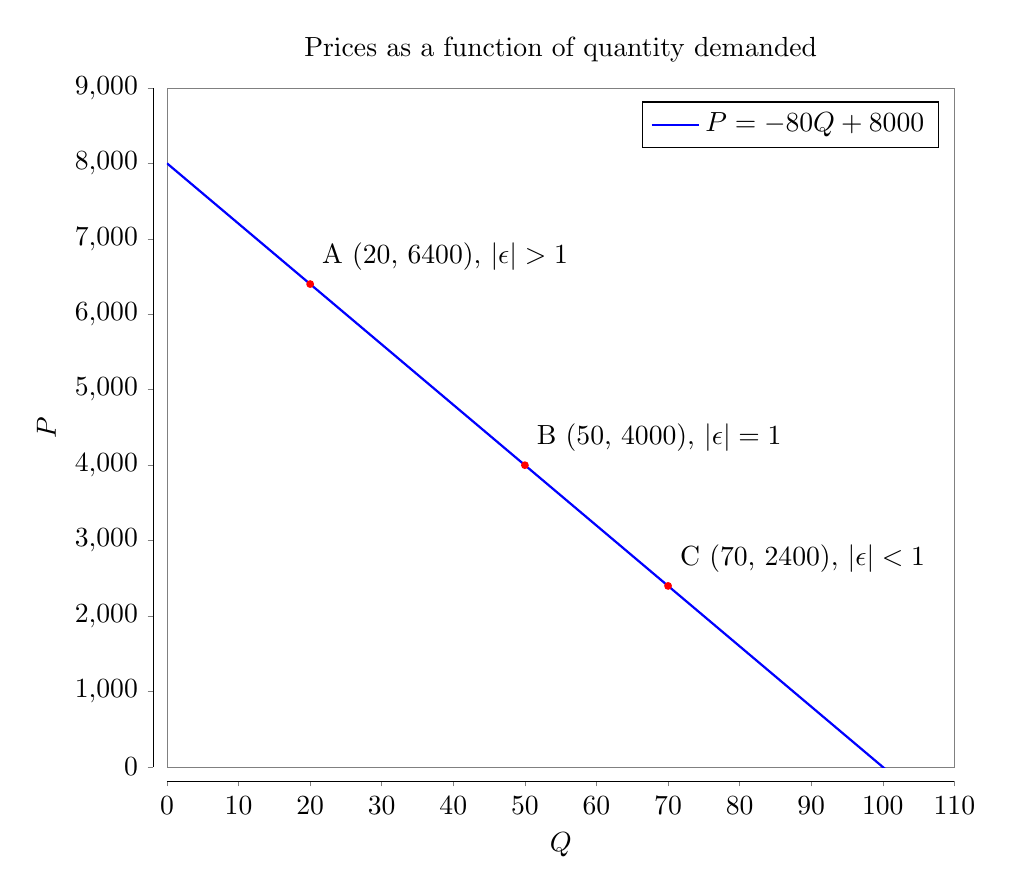
\begin{tikzpicture}

\begin{axis}[
    xmin = 0,
    xmax = 110,
    ymin = 0,
    ymax = 9000,
    xlabel = {$Q$},
    ylabel = {$P$},
    sciclean/.style={axis lines=left,
        axis x line shift=0.5em,
        axis y line shift=0.5em,
        axis line style={-,very thin},
        axis background/.style={draw,ultra thin,gray},
        tick align=outside,
        xtick distance=10,
        ytick distance=1000,
        major tick length=2pt},
    title = {Prices as a function of quantity demanded},
    sciclean]

\addplot[thick, color = blue, domain = 0:120] {-80*x + 8000};
\addlegendentry{$P = -80Q + 8000$}
\node[label = {60:A (20, 6400), $ |\epsilon| > 1 $}, fill=red,circle,inner sep=1pt] at (axis cs:20,6400) {} ;
\node[label = {60:B (50, 4000), $ |\epsilon| = 1$}, fill=red,circle,inner sep=1pt] at (axis cs:50,4000) {} ;
\node[label = {60:C (70, 2400), $ |\epsilon| < 1 $}, fill=red,circle,inner sep=1pt] at (axis cs:70,2400) {} ;

\end{axis}

    % We could control parts of figure only shown in beamer or vice versa.
    % \ifstandalone
    %     \node[below=1cm of mid] {Only Shown in Standalone Figure};
    % \else
    %     \node[below=1cm of mid] {Only Shown in Beamer};
    % \fi
\end{tikzpicture}

\end{document}
